\section{The hsMines Game}

As an example for more complex GUI programming, we will now develop a
GUI for a minesweeper like game called hsMines. Just in case you do
not know Minesweeper or some of its many clones I'll give a short
overview.

\subsection{What's that game?}
Playing Minesweeper you have a grid of about 20x20 similar
fields. Below any of this fields could be a mine or just an empty
field -- you wont know until you click at the field and are eventually
shred to pieces by some nasty mine. Goal of the game is to find all
the mines an mark them with tiny flags. An nearly impossible task. To
make the game any fun you are told the exact amount of mines around
the field you just opened. If this number is 0, it's safe to explore
all the adjacent fields. And because this is a stupid task the
machine does it for you. If you manage to explore all empty fields you
win, if you find one of the mines, you lost, best time gets the
highscore. Simple as that.

For this is not a course in haskell programming I will not spent any
words on the games code itself and will come straight to the very
heart of this section, the hsMines GUI.


\subsection{In the beginning\dots}
\dots, as you should have read, is the window. And for we are running
compiled code here, it's created in the \texttt{main} function.
\begin{code}
main = 
 do htk<- initHTk [withdrawMainWin]
    run htk normalSize 

run :: HTk-> (Int, Int)-> IO ()
run htk currentSize = 
 do main <- createToplevel [text "hsMines"]

finishHTk
\end{code}

Having only this, the GUI would look rather boring, but it's not bad
for just a few lines of code, isn't it? It looks a bit bent in a loop
but we will see later that this is needed to make the field
resizeable.\\
The last line is necessary to clean up all the events we've kicked
loose so far.

\begin{figure}[h]
\begin{center}
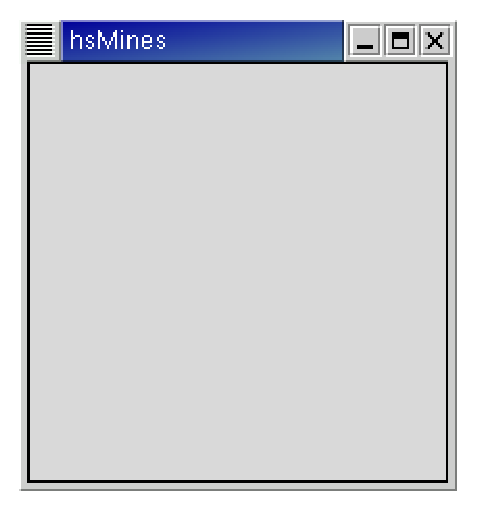
\includegraphics[scale=0.6]{img/Screenshot01}
\caption{The hsMines window}
\end{center}
\end{figure}

\subsection{Menus}

What would a GUI be without them? Somewhat empty as it seems. So let's
create some menus.

\begin{code}
    menubar <- createMenu main False []
    main # menu menubar

    fm <- createPulldownMenu menubar [text "File"]

    restb <- createMenuCommand fm [text "Restart"]
    qutib <- createMenuCommand fm [text "Quit"]

    pm <- createPulldownMenu menubar [text "Preferences"]
   
    pmc1 <- createMenuCascade pm [text "Size"]
    pmc1m <- createMenu main False []
    pmc1 # menu pmc1m
        
    pmc2 <- createMenuCascade pm [text "Difficulty"]
    pmc2m <- createMenu main False []
    pmc2 # menu pmc2m
\end{code}

To this point we create a number of menus and pulldowns. Let's go
through this step by step.
In line 1 we create an menu inside \emph{main} (our window) that was
created in \texttt{run}. In line 2 we tell \HTk to asign this new menu
we call \emph{menubar} to be the menu of \emph{main}.\\
In line 3 (we will not count the empty lines), we create our first
pulldown menu -- that is what actually is normaly called a menu. This
pulldown menu is created inside \emph{menubar}, is called \emph{fm}
and has the charming text "`File"'. For not leaving this menu (or
pulldown menu) empty, we create menu entrys so called menu commands
inside \emph{fm}. So by now we have \emph{restb} and \emph{quitb}
inside \emph{fm} inside \emph{menubar} inside \emph{main}.\\
This is quit nice but we will try to put some more functionality into
our menu besides restarting and quiting the game. And as we read
above, the game grid will be resizeable so we will need another menu
to have these commands in.\\
We create a second pulldown menu in \emph{menubar} called
\emph{pm}. In this menu we nest to submenus called menu
cascades. Each of the cascades has a name, \emph{pmc1} and
\emph{pmc2}, and a String set to it's text. The next step is a bit
tricky. One would expect now to fill the cascades directly with some
commands. But the menu cascades are only containers fit to hold a
menu. So we have to create another two menus inside main and asign
them to the two cascades. These two menus are called \emph{pmc1m} and
\emph{pmc2m} which should be an abreviation "`Prefernce Menu Cascade
1's Menu"' respectivly 2.\\
By now we have a menu which holds two pulldown menus. The
first contains two commands, the second contains two cascades which in
turn each contain a menu again. To make sense of these menus we have
to fill them of course. And finally we have to put some functions
behind those commands and what so ever or this would all be for
naught.

\begin{code}
    varSize <- createTkVariable currentSize
    sr1 <- createMenuRadioButton pmc1m [text "tiny (6x6)", value tinySize,
                                        variable varSize]
    sr2 <- createMenuRadioButton pmc1m [text "small (10x10)", value weeSize,
                                        variable varSize]
    sr3 <- createMenuRadioButton pmc1m [text "normal (15x15)", value normalSize,
                                        variable varSize]
    sr4 <- createMenuRadioButton pmc1m [text "large (20x20)", value bigSize,
                                        variable varSize]
    sr5 <- createMenuRadioButton pmc1m [text "huge (25x25)", value hugeSize,
                                        variable varSize]

    varDiff <- createTkVariable (6:: Int)
    dr1 <- createMenuRadioButton pmc2m [text "easy", value (8::Int),
                                        variable varDiff]
    dr2 <- createMenuRadioButton pmc2m [text "normal", value (6::Int),
                                        variable varDiff]
    dr3 <- createMenuRadioButton pmc2m [text "hard", value (4::Int),
                                        variable varDiff]
    dr4 <- createMenuRadioButton pmc2m [text "nuts", value (3::Int),
                                        variable varDiff]
\end{code}
In the code above we do several new things. First we create a new Tk
variable named \emph{varSize} and a few lines later one called
\emph{varDiff}. These are necessary to remember things we do to our
GUI like in this case switching a button.
Our next step is to create a menu radio button\footnote{
  A radio button is a button with several instances. Each of the
  instances is shown, can be selected and is bound to a different value
  but to the same variable. By selecting one of the instances the
  according value is asign to the variable. Because a variable can
  only have one value at a given time, only one of the instances can
  be selected.}
in each of the two submenus. The first radio button asigns tuples of
Int to the Variable \emph{varSize}, the actual values are given in a
couple of functions above in the code which can be fully seen in the
appendix.
% Hier beachten! Code muss in Appendix!
% Evtl. k�nnen die Funktionen auch wieder gel�scht und hier die
% konkreten Zahlen eingesetzt werden. Eigentlich m�ssten andernfalls
% die anderen Zahlen (f�r die Schwierigkeit) auch in Funktionen
% ausgelagert werden. So ist das inkonsequent.
As you we can see in the code above (in \texttt{main} and
\texttt{run}), currentSize holds the value of normalSize and so by
default the radio button is set to normalSize. Nearly the same happens
to \emph{varDiff} and it's radiobutton just without the hiding
functions.\\
The values of varDiff have to be explicitly casted because by default
TkVariables contain Strings. But still nothing happens besides setting
two varaibles.

\begin{code}
    restartClick <- clicked restb
    quitClick <- clicked quitb

    csr1 <- clicked sr1
    csr2 <- clicked sr2
    csr3 <- clicked sr3
    csr4 <- clicked sr4
    csr5 <- clicked sr5

\end{code}

This rather cryptic peace of codes allows us to bind the commands and
the size radio button(s) to a couple of events. These will occure now
whenever one of the buttons is selected -- "`clicked"'.

\begin{figure}[h]
\begin{center}
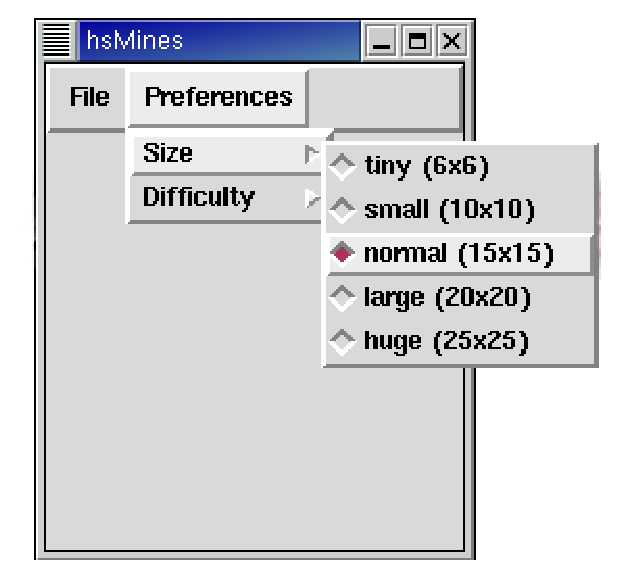
\includegraphics[scale=0.6]{img/Screenshot02}
\caption{The hsMines main window with an open Prefs/Size menu}
\end{center}
\end{figure}

\subsection{The field}

To make all the decoration perfect, wie need the little smiley atop
the playfield which can be used to restart the game.
\begin{code}
    sm <- newButton main [photo smSmileImg]
    startClick <- clicked sm

    pack sm [Side AtTop, PadY 20, PadX 20, Anchor North] 
\end{code}
So we create a Button called sm (from \textbf{sm}iley btw) and bind it
to another Event. And because the GUI does not automaticaly know where
and when to place the button we have to tell it to \texttt{pack sm at
the top of the main window, pad it 20 pixels wide in any direction
and keep it align to the upperside} (which is North on most maps). The
photo-Command assigns an Image to a Container that is fit to contain
an Image e.g. a button widget. In this case we have a collection of
base64 encoded GIFs pasted into the code. This is definitivly not the
best way to use graphics, but it works. As we will we later, there are
also tiny Images for the empty field and the numbers and not only the
flag. The reason for that is, that you can't overwrite a photo with
some text. We may do it internaly but it will not be shown. The
workaround is to have Images for all the numbers. On the other hand
we have a wide selection of colours for the numbers. Just try to find
out wich colour the '8' has\dots But back to the smiley.\\
Same as the menu commands, the buttons is useless by itself. To get
things started we create an IO-channel named restartCh. We can later
at any given time send some IO-signal over this channel to trigger an
event which will be used to reinitialise the game field.

\begin{code}
    restartCh <- newChannel
    allbuttons <- buttons bfr sm (receive restartCh) size
\end{code}

But before we can initialise any game field, we of course have to
create it. To contain the field we create a new Frame (a container
widget) with a given width. The width is just to have something to
start with and will be adjusted by the packer as needed. 
The Frame is packed below the smiley button. They both are told to be
at the top of main, but because only one of them can be there they're
placed below each other in packing order. 

\begin{code}
    bfr <- newFrame main [width (cm 10)]
    pack bfr [Side AtTop, PadX 15] 
\end{code}

Until now this was all very plain and straight. The buttons for the
field are created in a more complex way. The function
\texttt{buttons}, the one called with the IOChannel, is responsible to
create a number of buttons and asigns them to \emph{allbuttons}. To
pack them, we have to iterate through the whole list of buttons.

\begin{code}
    mapM_ (\(xy, b)-> grid b [GridPos xy, GridPadX 1, GridPadY 1]) allbuttons
\end{code}

In this case a grid packer is used that puts all the buttons at
exactly stated positions in a grid. So let's for now assume,
\texttt{buttons} returns a list of buttons that can be packed by the
grid packer. If the code compilation does not reach any point where
the game is started, the packed but uninitialised game field including
the smiley and all thing looks like this. To make a distinction
between uninitialised and initialised fields, we put a little star
image on each button.

\begin{figure}[h]
\begin{center}
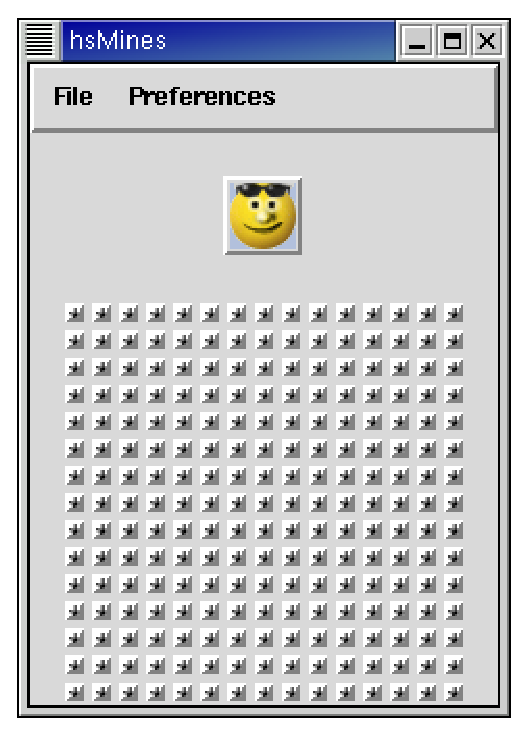
\includegraphics[scale=0.3]{img/Screenshot03}
\caption{The uninitialised hsMines field}
\end{center}
\end{figure}

All that is left to do now in \texttt{run} is to initiate the game for
the first time. 

\begin{code}
    let start :: IO () 
        start = do diff <- readTkVariable varDiff
                   sendIO restartCh diff
                   
    -- start the menu handler
    stopmh<- spawnEvent (forever (startClick >>> start
                               +> quitClick >>> destroy htk
                               +> choose [csr1, csr2, csr3, csr4, csr5] >>> 
                                           createMessageWin "Changes come into effect after \"Restart\"." []
                        ))

    -- the restart handler (note no forever!)
    spawnEvent (restartClick >>> do stopmh
                                    destroy main
                                    nuSize <- readTkVariable varSize
                                    run htk nuSize)

    -- start the game
    start

    -- wait for game to stop, then clear up the mess
    finishHTk

\end{code}

There is a bit more to clean up the window and such. We will see to
this now. Let us go through this step by step. \texttt{start} is a
function that returns an empty IO operation. Inside the functions, the
variable \emph{varDiff} which holds the games difficulty is read and
sent via the IOChannel \emph{restartCh}. This will take effect in
\texttt{buttons} and we'll come to this later. But \texttt{start} is
not the first thing to happen. First, an event is bound to
\emph{stopmh} but is not spawned instantly because haskell is
evaluated lazyly and so the evalutation will take place when
\emph{stopmh} is realy needed - which happens to be just in the next
line. There another event is spawned. This one immediately performes 4
functions. Now stopmh is evaluated and the event is spawned. The
second action is to destroy the \emph{main} window. Step 3 and 4
create a new window with the actual field size. This is the reason fpr
the intervined function calls of \texttt{run} and \texttt{main}.\\
The second event thread, that is spawned in step 1 now waits for a
number of things to happen. Either the startClick event occurs and
start is executed or the quitClick event occurs and the whole htk is
destroyed or on of the size selecting radiobuttons is clicked meaning
that one of the five csr events occurs which leads to the creation of
a message window.\\
Finally, at the end of the \texttt{run} function \texttt{start} is
called and the game is started. Remember? The size of the game field
is sent via restartCh and something will happen in \texttt{buttons}.
Let's take a look at
%This is NO typo but intentionaly done.

\subsection{The buttons function}

This function has a rather complex signature.

\begin{code}
buttons :: Container par=> par-> Button-> Event Int-> (Int, Int)
                           -> IO [((Int, Int), Button)]

\end{code}

For comparison lets have another look on how it's called:

\begin{code}
    allbuttons <- buttons bfr sm (receive restartCh) size
\end{code}

We have a class restriction on the first argument, \emph{par}, which
has to be a \emph{Container}. \emph{par} happens to be just that, a
\emph{Frame}. Lucky us. The next argument has to be a \emph{Button} as
we can happily admit our smiley buttons \emph{sm} is. The third
argument has to be an Event of Int. This Event occurs, when some IO
Int is send via the IO Channel \emph{restartCh} and is received by
\texttt{receive}. The last argument is a 2-tuple of Int which is the
size of the game field. \emph{size} is an Int read from the TkVariable
\emph{varSize}. So when something is asigned to \emph{allbuttons}, the
function \texttt{buttons} is called with a lot of intricate arguments.

When buttons has done it's work, it will return an IO of a list auf
tuples of tuples of Int and a Button. We can see that it is simpler to
examine the signature ourselfs than try to puzzle out what was just
told.

The code of buttons is simple at start.

\subsubsection{Create an array of buttons,\dots}

\begin{code}
buttons par sb startEv (size@(xmax, ymax)) =
  do buttons <- mapM (\xy-> do b<- newButton par [photo starImg, relief Raised]
                               return (xy, b)) [(x, y) | x <- [1.. xmax],
                                                         y <- [1.. ymax]]
\end{code}

This code is executed no matter what startEv might be! It creates all
the buttons and paints a little star inside so the playfield looks
the way the Figure above shows it.%Verweis auf Figure?
But there is more to happen in the buttons function!

\subsubsection{bind them\dots}

\begin{code}
     let bArr = array ((1,1), size) buttons
         getButtonClick b n xy = 
            do (click, _) <- bindSimple b (ButtonRelease (Just n))
               return (click >> return xy)
     leCl  <- mapM (\(xy, b)-> getButtonClick b 1 xy) buttons
     riCl  <- mapM (\(xy, b)-> getButtonClick b 3 xy) buttons
     press <- mapM (\(_, b)-> do (cl, _)<- bindSimple b (ButtonPress Nothing)
                                 return cl) buttons

\end{code}

This looks rather complicated but does nothing more than what we did,
when we bound the smiley button to the startClick Event. It's just
that we bind the whole Array of buttons we created via a slightly
adjusted Event (\texttt{getButtonClick b 1/3 xy})\footnote{ As you
  could surely guess, 2 would be the modifier to get the center button
  bound.  } to two Events. We also bind the Button to the \emph{press}
Event. This Event occurs whenever a Button is pressed. It's used to
alter the smiley and because it doesn't matter which Button is
pressed, we don't keep the coordinates. Know the programm knows,
whether a Button is clicked and, when it's released, which Button it
is and if it was clicked with the left or the right mouse button.
Funny thing is that if you use the middle mouse button to click a
Button, the smiley will stay worried.

\subsubsection{and start\dots}

\begin{code}
     spawnEvent start
     return buttons
\end{code}

At the end, we spawn an Event called start and wait. But wait what
for? We need to remember that an Event is handed over to
\texttt{buttons}. And this event is used to get the game running.

\begin{code}
         start :: Event ()
         start = startEv >>>= \d-> do m <- createMines (snd (bounds bArr)) d
                                      sb # photo smSmileImg
                                      mapM_ (\b-> b # photo zeroImg >>= 
                                                    relief Raised) (elems bArr)
                                      sync (play m)

\end{code}

This says: If the Event start occurs (by being spawned for example)
then startEv, if it occurs, executes some more code. Have a look on
how we create mines later, it's of no importance for the GUI. We map
over all elements in the Button Array \emph{bArr} and asign the
\emph{zeroImg} to their photo. Then we asign a new smiley to the photo
of \emph{sb} and synchronize the start Event to the play Event. No new
Event is created, start just changed into play.

\subsubsection{to play\dots}

\begin{code}
         play :: Mines-> Event ()
         play m = do r <- choose leCl >>>= open bArr m
                     case r of Nothing -> always gameLost >> gameOver
                               Just nu -> -- for simplicity, we have won
                                          -- if no untouched fields are left
                                          if all (not.untouched)
                                                           (elems nu) then 
                                            always gameWon >> gameOver
                                          else playOn nu
                  +>
                  do r<- choose riCl >>>= flag bArr m
                     playOn r
                  +>
                  -- make smiley frown when we press a mouse button
                  do choose press 
                     always (sb # photo smWorriedImg >> done) 
                     play m
                  +>
                  start 

\end{code}

Playing is easy. To play with a set m of mines means to execute these
steps over and over again:

\begin{enumerate}
\item If the left mousebutton is pressed, execute \texttt{open} with
  the Button Array and the mines. If Nothing is left, you
  loose\footnote{ Of course this is the case because \texttt{open}
    returns Nothing if we try to explore a mine.}  If there are mines
  left, you play on. And if all fields are explored we won. Great,
  isn't it?
\item If the right mousebutton is pressed, execute \texttt{flag} with
  the Button Array and the mines. No evil may occur, just play on.
\item If a mouse button is pressed (remember, even the middle button
  counts), the smiley should look worried. Normaly another Event
  occurs so the smiley changes within a second but only if we pressed
  the left or right mouse button. This, of course, is a feature.
\item If thing go awry, goto start and wait for the startEv Event.
\end{enumerate}

\begin{code}
         playOn :: Mines-> Event ()
         playOn m = do always (sb # photo smCoolImg)
                       play m       
\end{code}

\texttt{playOn} takes care of the smiley when we (de)flaged some field
or explored it.

\subsubsection{until it's over.}

\texttt{gameLost} and \texttt{gameWon} are just Windows to open,
to tell you that you've lost or won. That also changes your smiley
into a freak.

\begin{code}
         gameLost :: IO ()
         gameLost = do sb # photo smSadImg
                       createAlertWin "*** BOOM!***\nYou lost." []
         gameWon :: IO ()
         gameWon = do  sb # photo smWinImg
                       createMessageWin "You have won!" []

\end{code}

Only after you finished up the messenger, the game is realy over and
can be started again, the \verb�>>� operator takes care of that.

\begin{code}
         gameOver :: Event ()
         gameOver = start 
                    +> 
                    (choose (leCl++ riCl) >> gameOver) 
\end{code}

\texttt{gameOver} is the Event to take over. It leads you back to the
start event, waiting for the \emph{startEv} Event to occur. If any of
the ingame Events occur, because some dumbhead did not understand the
"`BOOM! You lost."' message or what so ever, the game is still over
and nothing changes.

That's it, anything else is just plain haskell. Naugh, you're right,
there is some tiny tidbits left. Nobody explained how the numbers show
up when a non mine field is explored, right? Okay, we'll come to that
now.

\subsection{Fuzzing around on the play field}

The simple part is leaving and taking flags.

\begin{code}
flag :: Buttons-> Mines-> (Int, Int)-> IO Mines
flag b m xy = 
  case m!xy of
    Cleared _ -> return m
    s@(Unexplored{flagged= f})-> 
        do b!xy # (if not f then photo flagImg else photo zeroImg)
           return (m // [(xy, s{flagged= not f})])
\end{code}

The function takes the Button Array, the Mines and the coordinates of
the selected button. If the the field is Cleared which means it was
explored more early the Mines are simply returned. If the field is
Unexplored and flagged we set it unflagged and asign the
\emph{zeroImg} to its Button and vice versa.

The more complex part is actually exploring the field.

\begin{code}
open :: Buttons-> Mines-> (Int, Int)-> IO (Maybe Mines)
open b m xy = 
  case m!xy of 
    Cleared _                  -> return (Just m)
    Unexplored {flagged= True} -> return (Just m)
    Unexplored {mine= True}    -> return Nothing
    _ -> peek b m [xy] >>= return. Just
\end{code}

The function takes the same arguments but it only may return IO Mines.
If we try to explore an Cleared field, nothing changes. If we try to
explore an Unexplored field which is flagged, we return the given
argument and still nothing changes. If we try to open an Unexplored
field which is a mine the function returns Nothing wich leads to
\texttt{gameLost} in \texttt{buttons}. And at last, when every other
case is weeded out, we \texttt{peek} inside an Unexplored, nonflagged
nomine field.

\begin{code}
peek :: Buttons-> Mines-> [(Int, Int)]-> IO Mines
peek b m [] = return m
peek b m (xy:rest) =
   let adjMines :: Int
       adjMines = sum (map (mines. (m !)) (adjacents m xy))
       nu       = m // [(xy, Cleared adjMines)]
   in do (b!xy)# photo (getImg adjMines) >>= relief Flat
         if adjMines == 0 then 
            peek b nu (rest `union` (filter (untouched. (m !))
                                            (adjacents m xy)))
            else peek b nu rest
\end{code}

\texttt{peek} takes a list of coordinates to check. Initially this
should be exactly one coordinate respectivly the one we try to explore
right now. We use \texttt{adjMines} the get the number of mines around
the field to explore wich is a number from 0 to 8. We asign the
corresponding Image to the Button's photo and change its relief to
Flat. In case the number is not 0, this would just be it because now
the list of coordinates would be empty. But to make life more
comfortable we will now use the computer for its main purpose: To
accomplish stupid tasks for us. Because if the number of mines in the
adjacent fields is 0 we can savely explore any of these. So now
\emph{rest}, the list of coordinates still to explore (an empty list
right now) is unified with the coordinates of the adjecent fields
which are still Unexplored. If we forgot to apply this filter the
exploration would go on forever exploring the same fields over and
over again. But if it's done right the programm explores all save
fields thereby creating number rimmed empty areas on the playfield.

\begin{figure}[h]
\begin{center}
\includegraphics[scale=0.3]{img/Screenshot04}
\caption{The hsMines field after a single lucky Click}
\end{center}
\end{figure}

\begin{figure}[h]
\begin{center}
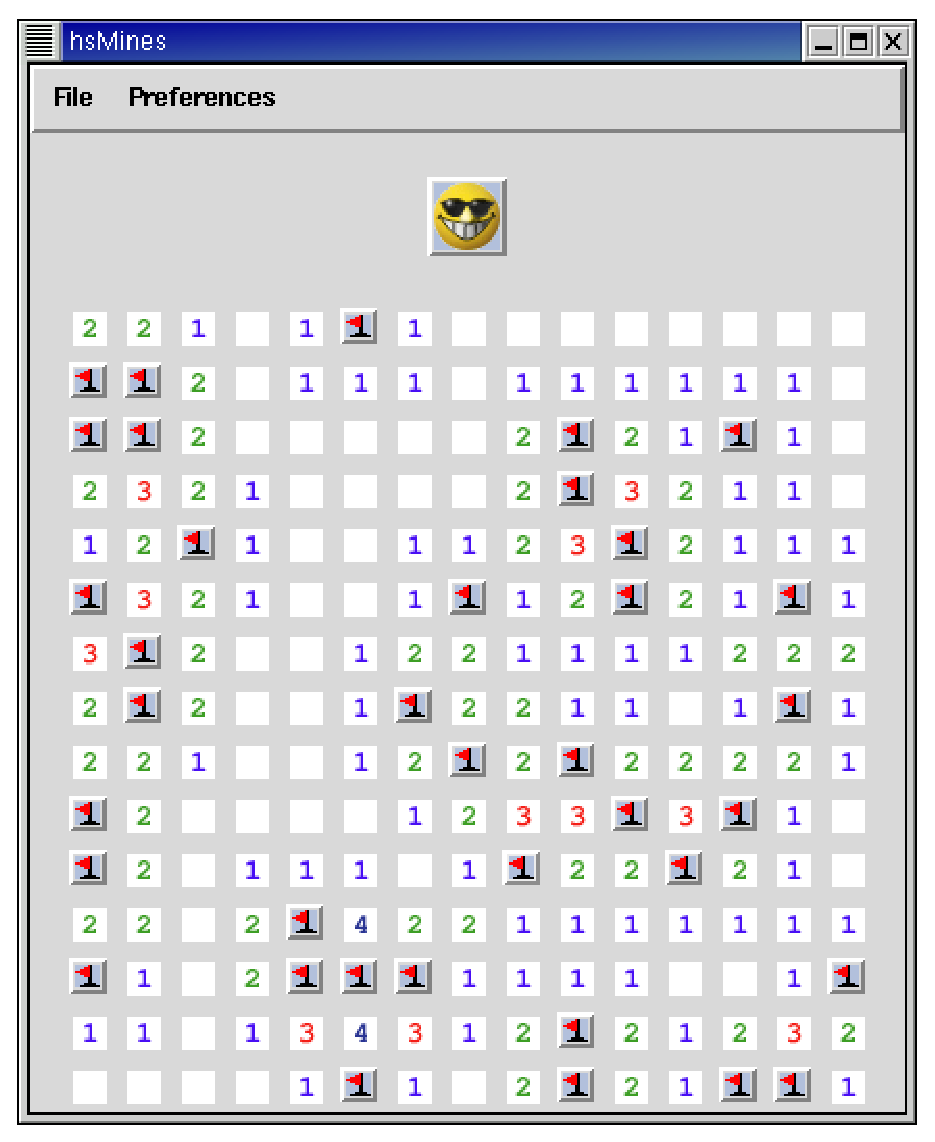
\includegraphics[scale=0.3]{img/Screenshot05}
\caption{The same field a few lucky Clicks later}
\end{center}
\end{figure}



%%% Local Variables: 
%%% mode: latex
%%% TeX-master: "intro"
%%% End: 

